
%(BEGIN_QUESTION)
% Copyright 2006, Tony R. Kuphaldt, released under the Creative Commons Attribution License (v 1.0)
% This means you may do almost anything with this work of mine, so long as you give me proper credit

A very bored and overpaid instrument technician decides to equip her hot tub with this temperature control system, which works by varying the ratio of hot to cold water added to the tub:

$$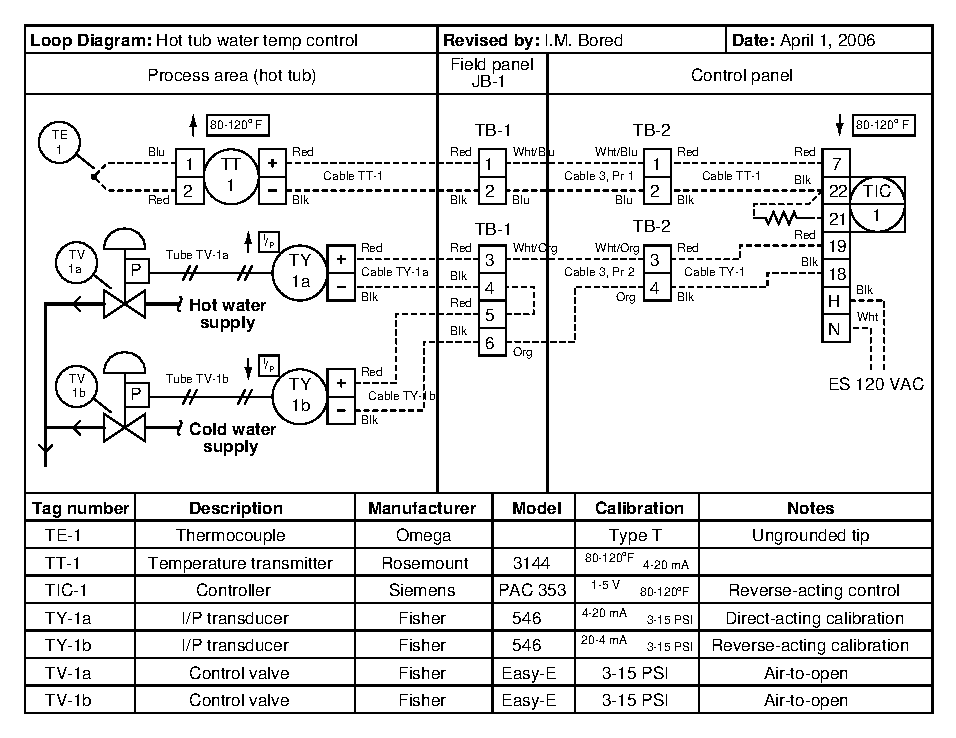
\includegraphics[width=15.5cm]{i01397x01.eps}$$

Examine this loop diagram closely, and then answer the following questions:

\begin{itemize}
\item{} Where does the ``split-ranging'' (sequencing) take place in this system?
\vskip 10pt
\item{} What will happen in the event that cable 3 becomes completely severed?
\vskip 10pt
\item{} What will happen in the event of total instrument air pressure loss?
\vskip 10pt
\item{} Determine the positions of both valves at a controller output signal of 13.5 mA.
\vskip 10pt
\item{} How much voltage will the controller have to output between terminals 19 and 18 when the output signal is at 100\% of range?  Assume a coil resistance of 176 ohms for each of the model 546 I/P transducers.
\end{itemize}

\vskip 20pt \vbox{\hrule \hbox{\strut \vrule{} {\bf Suggestions for Socratic discussion} \vrule} \hrule}

\begin{itemize}
\item{} Identify an alternative scheme for accomplishing the same sequence of split-ranging.  In other words, wherever the split-range sequencing happens in this system, devise a way the sequencing could be done in different components.
\end{itemize}

\underbar{file i01397}
%(END_QUESTION)





%(BEGIN_ANSWER)

\noindent
{\bf Partial answer:}

\begin{itemize}
%\item{} Where does the ``split-ranging'' take place in this system? {\bf In the I/P transducers.}
%\vskip 10pt
\item{} What will happen in the event that cable 3 becomes completely severed? {\bf The hot water valve will completely shut and the cold water valve will completely open.}
%\vskip 10pt
%\item{} What will happen in the event of total instrument air pressure loss? {\bf No water (cold or hot) will go into the hot tub.}
%\vskip 10pt
%\item{} Determine the positions of both valves at a controller output signal of 13.5 mA. {\bf Hot water valve 59.375\% open ; cold water valve 40.625\% open.}
\vskip 10pt
\item{} How much voltage will the controller have to output between terminals 19 and 18 when the output signal is at 100\% of range?  Assume a coil resistance of 176 ohms for each of the model 546 I/P transducers.  {\bf 7.04 volts DC}
\end{itemize}
 
%(END_ANSWER)





%(BEGIN_NOTES)

This is the type of split-ranging used in this system:

$$\includegraphics[width=15.5cm]{i01397x02.eps}$$

\begin{itemize}
\item{} Where does the ``split-ranging'' take place in this system? {\bf In the I/P transducers.}
\vskip 10pt
\item{} What will happen in the event that cable 3 becomes completely severed? {\bf The hot water valve will completely shut and the cold water valve will completely open.}
\vskip 10pt
\item{} What will happen in the event of total instrument air pressure loss? {\bf No water (cold or hot) will go into the hot tub.}
\vskip 10pt
\item{} Determine the positions of both valves at a controller output signal of 13.5 mA. {\bf Hot water valve 59.375\% open ; cold water valve 40.625\% open.}
\vskip 10pt
\item{} How much voltage will the controller have to output between terminals 19 and 18 when the output signal is at 100\% of range?  Assume a coil resistance of 176 ohms for each of the model 546 I/P transducers.  {\bf 7.04 volts DC}
\end{itemize}






 
\vskip 20pt \vbox{\hrule \hbox{\strut \vrule{} {\bf Virtual Troubleshooting} \vrule} \hrule}

This question is a good candidate for a ``Virtual Troubleshooting'' exercise.  Presenting the diagram to students, you first imagine in your own mind a particular fault in the system.  Then, you present one or more symptoms of that fault (something noticeable by an operator or other user of the system).  Students then propose various diagnostic tests to perform on this system to identify the nature and location of the fault, as though they were technicians trying to troubleshoot the problem.  Your job is to tell them what the result(s) would be for each of the proposed diagnostic tests, documenting those results where all the students can see.

During and after the exercise, it is good to ask students follow-up questions such as:

\begin{itemize}
\item{} What does the result of the last diagnostic test tell you about the fault?
\item{} Suppose the results of the last diagnostic test were different.  What then would that result tell you about the fault?
\item{} Is the last diagnostic test the best one we could do?
\item{} What would be the ideal order of tests, to diagnose the problem in as few steps as possible?
\end{itemize}

%INDEX% Final Control Elements, valve: split ranging
%INDEX% Process: hot tub temperature control

%(END_NOTES)


